
%%%%%%%%%%%%%%%%%%%%%%%%%%%%%%%%%%%%%%%%%%%%%%%%%%%%%%%%%%%%%%%%%%
%%%%%%%%%%%%%%%%%%%%%%%%%%%%%%%%%%%%%%%%%%%%%%%%%%%%%%%%%%%%%%%%%%
%Packages
\documentclass[10pt, a4paper]{article}
\usepackage[top=3cm, bottom=4cm, left=3.5cm, right=3.5cm]{geometry}
\usepackage{amsmath,amsthm,amsfonts,amssymb,amscd, fancyhdr, color, comment, graphicx, environ}
\usepackage{float}
\usepackage{mathrsfs}
\usepackage[math-style=ISO]{unicode-math}
% \setmathfont{TeX Gyre Termes Math}
\usepackage{lastpage}
\usepackage[dvipsnames]{xcolor}
\usepackage[framemethod=TikZ]{mdframed}
\usepackage{enumerate}
\usepackage[shortlabels]{enumitem}
\usepackage{fancyhdr}
\usepackage{indentfirst}
\usepackage{listings}
\usepackage{sectsty}
\usepackage{thmtools}
\usepackage{shadethm}
\usepackage{hyperref}
\usepackage{setspace}
\hypersetup{
    colorlinks=true,
    linkcolor=blue,
    filecolor=magenta,      
    urlcolor=blue,
}
%%%%%%%%%%%%%%%%%%%%%%%%%%%%%%%%%%%%%%%%%%%%%%%%%%%%%%%%%%%%%%%%%%
%%%%%%%%%%%%%%%%%%%%%%%%%%%%%%%%%%%%%%%%%%%%%%%%%%%%%%%%%%%%%%%%%%
%Environment setup
\mdfsetup{skipabove=\topskip,skipbelow=\topskip}
\newrobustcmd\ExampleText{%
An \textit{inhomogeneous linear} differential equation has the form
\begin{align}
L[v ] = f,
\end{align}
where $L$ is a linear differential operator, $v$ is the dependent
variable, and $f$ is a given non−zero function of the independent
variables alone.
}
\mdfdefinestyle{theoremstyle}{%
linecolor=black,linewidth=1pt,%
frametitlerule=true,%
frametitlebackgroundcolor=gray!20,
innertopmargin=\topskip,
}
\mdtheorem[style=theoremstyle]{Problem}{Problem}
\newenvironment{Solution}{\textbf{Solution.}}

\definecolor{codegreen}{rgb}{0,0.6,0}
\definecolor{codegray}{rgb}{0.5,0.5,0.5}
\definecolor{codepurple}{rgb}{0.58,0,0.82}
\definecolor{backcolour}{rgb}{0.95,0.95,0.92}

\lstdefinestyle{mystyle}{
    backgroundcolor=\color{backcolour},   
    commentstyle=\color{codegreen},
    keywordstyle=\color{magenta},
    numberstyle=\tiny\color{codegray},
    stringstyle=\color{codepurple},
    basicstyle=\ttfamily\footnotesize,
    breakatwhitespace=false,         
    breaklines=true,                 
    captionpos=b,                    
    keepspaces=true,                 
    numbers=left,                    
    numbersep=5pt,                  
    showspaces=false,                
    showstringspaces=false,
    showtabs=false,                  
    tabsize=2
}

\lstset{style=mystyle}
%%%%%%%%%%%%%%%%%%%%%%%%%%%%%%%%%%%%%%%%%%%%%%%%%%%%%%%%%%%%%%%%%%
%%%%%%%%%%%%%%%%%%%%%%%%%%%%%%%%%%%%%%%%%%%%%%%%%%%%%%%%%%%%%%%%%%
%Fill in the appropriate information below
\newcommand{\norm}[1]{\left\lVert#1\right\rVert}     
\newcommand\course{CS550 Machine Learning}                            % <-- course name   
\newcommand\hwnumber{ 4}                                 % <-- homework number
\newcommand\Information{Karan Sunil Kumbhar }                        % <-- personal information
\newcommand\Informatio{Id. - 12140860}
\newcommand\Informati{BTech CSE}
\newcommand\Informat{2025}
%%%%%%%%%%%%%%%%%%%%%%%%%%%%%%%%%%%%%%%%%%%%%%%%%%%%%%%%%%%%%%%%%%
%%%%%%%%%%%%%%%%%%%%%%%%%%%%%%%%%%%%%%%%%%%%%%%%%%%%%%%%%%%%%%%%%%
%Page setup
\pagestyle{fancy}
\headheight 35pt
\lhead{\today}
\rhead{
\includegraphics[width=2.0cm]{iitbh.png}}
\lfoot{}
\pagenumbering{arabic}
\cfoot{\small\thepage}
\rfoot{}
\headsep 2.7em
\renewcommand{\baselinestretch}{1.25}
%%%%%%%%%%%%%%%%%%%%%%%%%%%%%%%%%%%%%%%%%%%%%%%%%%%%%%%%%%%%%%%%%%
%%%%%%%%%%%%%%%%%%%%%%%%%%%%%%%%%%%%%%%%%%%%%%%%%%%%%%%%%%%%%%%%%%
%Add new commands here
\renewcommand{\labelenumi}{\alph{enumi})}
\newcommand{\Z}{\mathbb Z}
\newcommand{\R}{\mathbb R}
\newcommand{\Q}{\mathbb Q}
\newcommand{\NN}{\mathbb N}
\newcommand{\PP}{\mathbb P}
\DeclareMathOperator{\Mod}{Mod} 
\renewcommand\lstlistingname{Algorithm}
\renewcommand\lstlistlistingname{Algorithms}
\def\lstlistingautorefname{Alg.}
\newtheorem*{theorem}{Theorem}
\newtheorem*{lemma}{Lemma}
\newtheorem{case}{Case}
\newcommand{\assign}{:=}
\newcommand{\infixiff}{\text{ iff }}
\newcommand{\nobracket}{}
\newcommand{\backassign}{=:}
\newcommand{\tmmathbf}[1]{\ensuremath{\boldsymbol{#1}}}
\newcommand{\tmop}[1]{\ensuremath{\operatorname{#1}}}
\newcommand{\tmtextbf}[1]{\text{{\bfseries{#1}}}}
\newcommand{\tmtextit}[1]{\text{{\itshape{#1}}}}

\newenvironment{itemizedot}{\begin{itemize} \renewcommand{\labelitemi}{$\bullet$}\renewcommand{\labelitemii}{$\bullet$}\renewcommand{\labelitemiii}{$\bullet$}\renewcommand{\labelitemiv}{$\bullet$}}{\end{itemize}}
\catcode`\<=\active \def<{
\fontencoding{T1}\selectfont\symbol{60}\fontencoding{\encodingdefault}}
\catcode`\>=\active \def>{
\fontencoding{T1}\selectfont\symbol{62}\fontencoding{\encodingdefault}}
\catcode`\<=\active \def<{
\fontencoding{T1}\selectfont\symbol{60}\fontencoding{\encodingdefault}}

%%%%%%%%%%%%%%%%%%%%%%%%%%%%%%%%%%%%%%%%%%%%%%%%%%%%%%%%%%%%%%%%%%
%%%%%%%%%%%%%%%%%%%%%%%%%%%%%%%%%%%%%%%%%%%%%%%%%%%%%%%%%%%%%%%%%%
%Begin now!
\begin{document}

\begin{titlepage}
    \begin{center}
        \vspace*{3cm}

        \Huge
        \textbf{Machine Learning}

        \vspace{1cm}
        \huge
        Homework\hwnumber

        \vspace{1.5cm}
        \Large

        \textbf{\Information}\\                      % <-- author
        \textbf{\Informatio}\\
        \textbf{\Informati} \\
        \textbf{\Informat} \\

        \vfill

        \course \

        \vspace{1cm}

        
\includegraphics[width=0.4\textwidth]{iitbh.png}
        \\

        \Large

        \today

    \end{center}
\end{titlepage}


%%%%%%%%%%%%%%%%%%%%%%%%%%%%%%%%%%%%%%%%%%%%%%%%%%%%%%%%%%%%%%%%%%
% Example of referring to a piece of code.
% \lstinputlisting[language = python]{Program Solution.py}
%%%%%%%%%%%%%%%%%%%%%%%%%%%%%%%%%%%%%%%%%%%%%%%%%%%%%%%%%%%%%%%%%%
%Start the assignment now
%%%%%%%%%%%%%%%%%%%%%%%%%%%%%%%%%%%%%%%%%%%%%%%%%%%%%%%%%%%%%%%%%%
%New problem
\newpage
\subsubsection*{}

\begin{Problem}
    \textbf{Ch10\_Q1}
\end{Problem}

\begin{Solution}

    \begin{enumerate}[label=\textbf{(\alph*)}]
        \item
              Neural network described with p = 4 input units, 2 units in the first hidden layer, 3 units in the second hidden layer, and a single output
              \begin{mdframed}
                  \begin{center}
                      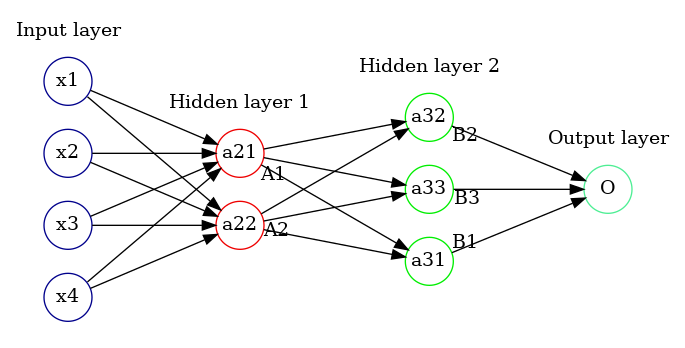
\includegraphics[scale=0.5]{graph.png}
                  \end{center}
              \end{mdframed}

        \item
              Assinging weights and biases to each nueron whcih is shown in below figure 1

              \begin{figure}[h]
                  \caption{Assinging weights and biases}
                  \begin{mdframed}
                      \begin{minipage}{0.45\textwidth}
                          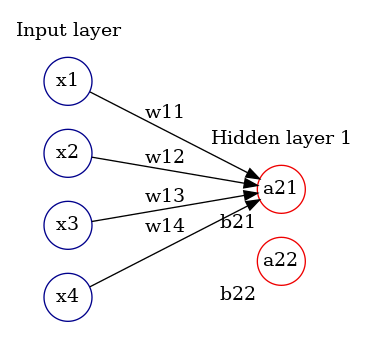
\includegraphics[width=\linewidth]{l1p1.png}
                      \end{minipage}\hfill
                      \begin{minipage}{0.45\textwidth}
                          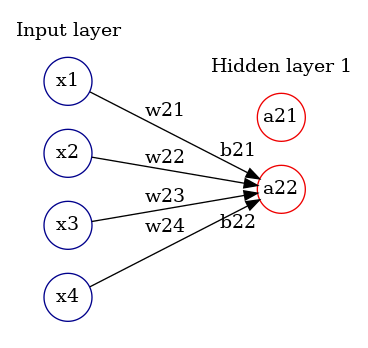
\includegraphics[width=\linewidth]{l1p2.png}
                      \end{minipage}

                      \vspace{1cm}

                      \begin{minipage}{0.45\textwidth}
                          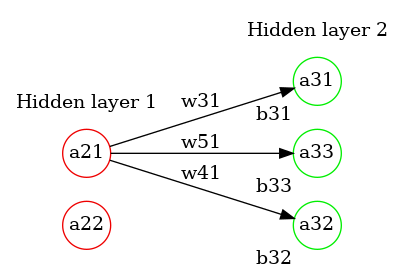
\includegraphics[width=\linewidth]{l2p1.png}
                      \end{minipage}\hfill
                      \begin{minipage}{0.45\textwidth}
                          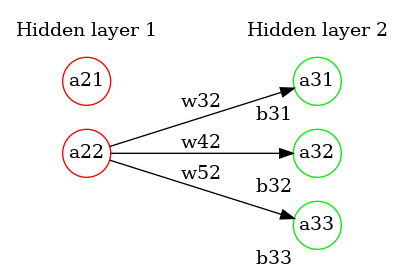
\includegraphics[width=\linewidth]{l2p2.png}
                      \end{minipage}
                  \end{mdframed}
              \end{figure}

              Let's break down the calculations step by step. We'll assume ReLU activation functions and denote weights as $w_i$ and biases as $b_i$ for simplicity.

              \textbf{Step 1:} Calculating the inputs for the first hidden layer:
              \begin{align*}
                  \text{Input to } a_{21} & = (x_1 \cdot w_{11}) + (x_2 \cdot w_{12}) + (x_3 \cdot w_{13}) + (x_4 \cdot w_{14}) + b_{21} \\
                  \text{Input to } a_{22} & = (x_1 \cdot w_{21}) + (x_2 \cdot w_{22}) + (x_3 \cdot w_{23}) + (x_4 \cdot w_{24}) + b_{22}
              \end{align*}

              \textbf{Step 2:} Applying the ReLU activation function to the inputs:
              \begin{align*}
                  A_{1} & = \text{ReLU(Input to } a_{21}) \\
                  A_{2} & = \text{ReLU(Input to } a_{22})
              \end{align*}

              \textbf{Step 3:} Calculating the inputs for the second hidden layer using the activations from the first hidden layer:
              \begin{align*}
                  \text{Input to } a_{31} & = (A_1 \cdot w_{31}) + (A_2 \cdot w_{32}) + b_{31} \\
                  \text{Input to } a_{32} & = (A_1 \cdot w_{41}) + (A_2 \cdot w_{42}) + b_{32} \\
                  \text{Input to } a_{33} & = (A_1 \cdot w_{51}) + (A_2 \cdot w_{52}) + b_{33}
              \end{align*}
              \newpage
              \textbf{Step 4:} Applying the ReLU activation function to the inputs:
              \begin{align*}
                  B_1 & = \text{ReLU(Input to } a_{31}) \\
                  B_2 & = \text{ReLU(Input to } a_{32}) \\
                  B_3 & = \text{ReLU(Input to } a_{33})
              \end{align*}

              Now, we have the outputs of the second hidden layer as $B_1$, $B_2$, and $B_3$ in terms of $x_1$, $x_2$, $x_3$, $x_4$, weights ($w$), and biases ($b$).

              \textbf{Step 5:} Calculating  the input to the output layer using the activations from the second hidden layer:
              \begin{align*}
                  \text{Input to } O & = (B_1 \cdot w_{61}) + (B_2 \cdot w_{62}) + (B_3 \cdot w_{63}) + b_{4}
              \end{align*}

              \textbf{Step 6:} Applying the ReLU activation function to obtain the final output $O$:
              \begin{align*}
                  f(x) & = \text{ReLU(Input to } O)
              \end{align*}
              \pagebreak

              So, the final output $f(x)$ is a function of the weights ($w_i$),($x_i$) and biases ($b_i$) for all layers, as well as the ReLU activation functions applied to the intermediate inputs.

        \item
              Let's put in some values for the coefficients and calculating the value of \( f(X) \). We'll assume the following coefficients:

              For the first hidden layer:
              \begin{align*}
                  w_{11} & = 0.5, \quad w_{12}   = -0.3, \quad w_{13}  = 0.2, \quad w_{14}  = 0.1,  \\
                  w_{21} & = -0.1, \quad w_{22}  = 0.2, \quad w_{23}   = 0.4, \quad w_{24}  = -0.2, \\
                  b_{21} & = 0.2, \quad b_{22}   = 0.1.
              \end{align*}

              For the second hidden layer:
              \begin{align*}
                  w_{31} & = 0.3, \quad w_{32}   = -0.1, \quad b_{31}  = 0.1,  \\
                  w_{41} & = -0.2, \quad w_{42}  = 0.3, \quad b_{32}   = -0.1, \\
                  w_{51} & = 0.2, \quad w_{52}   = 0.1, \quad b_{33}   = 0.2.
              \end{align*}

              For the output layer:
              \begin{align*}
                  w_{61} & = -0.3, \quad w_{62}  = 0.2, \quad w_{63}  = -0.1, \quad b_{4}  = 0.3.
              \end{align*}

              Now, let's calculate the value of \( f(X) \) by following the steps mentioned in part (b) with these coefficient values. We'll substitute the given coefficients into the equations for each layer to obtain the final output \( f(X) \).

              \begin{align*}
                  \text{Input to } a_{21} & = (x_1 \cdot 0.5) + (x_2 \cdot (-0.3)) + (x_3 \cdot 0.2) + (x_4 \cdot 0.1) + 0.2    \\
                                          & = 0.5x_1 - 0.3x_2 + 0.2x_3 + 0.1x_4 + 0.2                                           \\
                                          & =  0.5\cdot(1) - 0.3\cdot(1) + 0.2(1) + 0.1\cdot(1) + 0.2                           \\
                                          & = 0.7                                                                               \\
                  \text{Input to } a_{22} & = (x_1 \cdot (-0.1)) + (x_2 \cdot 0.2) + (x_3 \cdot 0.4) + (x_4 \cdot (-0.2)) + 0.1 \\
                                          & = -0.1x_1 + 0.2x_2 + 0.4x_3 - 0.2x_4 + 0.1                                          \\
                                          & = -0.1\cdot(1) + 0.2\cdot(1) + 0.4\cdot(1) - 0.2\cdot(1) + 0.1                      \\
                                          & = 0.4
              \end{align*}

              Now, Applying the ReLU activation function to the inputs:
              \begin{align*}
                  A_1 & = \max(0, 0.7) \\
                      & =  0.7         \\
                  A_2 & = \max(0, 0.4) \\
                      & = 0.4          \\
              \end{align*}

              For the second hidden layer :
              \begin{align*}
                  \text{Input to } a_{31} & = (A_1 \cdot 0.3) + (A_2 \cdot (-0.1)) + 0.1 \\
                                          & = 0.3A_1 - 0.1A_2 + 0.1                      \\
                                          & = 0.3\cdot(0.7) - 0.1\cdot(0.4)+ 0.1         \\
                                          & = 0.21 - 0.04 + 0.1                          \\
                                          & = 0.27                                       \\
                  \text{Input to } a_{32} & = (A_1 \cdot (-0.2)) + (A_2 \cdot 0.3) - 0.1 \\
                                          & = -0.2A_1 + 0.3A_2 - 0.1                     \\
                                          & = -0.2\cdot(0.7) + 0.3\cdot(0.4) - 0.1       \\
                                          & = -0.14 + 0.12 - 0.1                         \\
                                          & = - 0.12                                     \\
                  \text{Input to } a_{33} & = (A_1 \cdot 0.2) + (A_2 \cdot 0.1) + 0.2    \\
                                          & = 0.2A_1 + 0.1A_2 + 0.2                      \\
                                          & = 0.2\cdot(0.7) + 0.1\cdot(0.4) + 0.2        \\
                                          & = 0.14 + 0.04 + 0.2                          \\
                                          & = 0.38
              \end{align*}

              Applying the ReLU activation function to the inputs:
              \begin{align*}
                  B_1 & = \max(0, 0.27) \quad = 0.27 \\
                  B_2 & = \max(0, -0.12) \quad = 0   \\
                  B_3 & = \max(0, 0.38)\quad = 0.38
              \end{align*}

              Now, for the output layer, use the activations from the second hidden layer:
              \begin{align*}
                  \text{Input to } O & = (B_1 \cdot (-0.3)) + (B_2 \cdot 0.2) + (B_3 \cdot (-0.1)) + 0.3 \\
                                     & = -0.3B_1 + 0.2B_2 - 0.1B_3 + 0.3                                 \\
                                     & = -0.3\cdot(0.27) + 0.2\cdot(0) - 0.1\cdot(0.38) + 0.3            \\
                                     & = 0.181
              \end{align*}

              Finally, apply the ReLU activation function to obtain the final output \( O \):
              \begin{align*}
                  f(x) & = \max(0, 0.181) \\
                  f(x) & = 0.181
              \end{align*}

        \item
              \textbf{Number of Parameters:}

              To calculate the number of parameters in the neural network, we need to count the weights and biases. Here's the breakdown:

              \begin{itemize}
                  \item \textbf{First Hidden Layer:}
                        \begin{itemize}
                            \item 2 neurons in the first hidden layer.
                            \item Each neuron has 4 weights ($w_{11}, w_{12}, w_{13}, w_{14}$) and 1 bias ($b_{21}$).
                            \item Total parameters for the first hidden layer: $2 \times (4 \text{ weights} + 1 \text{ bias}) = 10$ parameters.
                        \end{itemize}

                  \item \textbf{Second Hidden Layer:}
                        \begin{itemize}
                            \item 3 neurons in the second hidden layer.
                            \item Each neuron has 2 weights ($w_{31}, w_{32}$) and 1 bias ($b_{31}$).
                            \item Total parameters for the second hidden layer: $3 \times (2 \text{ weights} + 1 \text{ bias}) = 9$ parameters.
                        \end{itemize}

                  \item \textbf{Output Layer:}
                        \begin{itemize}
                            \item 1 neuron in the output layer.
                            \item This neuron has 3 weights ($w_{61}, w_{62}, w_{63}$) and 1 bias ($b_{4}$).
                            \item Total parameters for the output layer: $1 \times (3 \text{ weights} + 1 \text{ bias}) = 4$ parameters.
                        \end{itemize}
              \end{itemize}

              Now, sum up the parameters from all layers:
              \begin{align*}
                  \text{Total Parameters} & = \text{Parameters in the first hidden layer}  \\
                                          & + \text{Parameters in the second hidden layer} \\
                                          & + \text{Parameters in the output layer}        \\
                                          & = 10 + 9 + 4                                   \\
                                          & = 23 \text{ parameters}
              \end{align*}

              So, there are a total of 23 parameters in this neural network.

    \end{enumerate}
\end{Solution}

%%%%%%%%%%%%%%%%%%%%%%%%%%%%%%%%%%%%%%%%%%%%%%%%%%%%%%%%%%%%%%%%%%
%New problem
\newpage
\subsubsection*{}
\begin{Problem}
    \textbf{Ch10\_Q2}
\end{Problem}

\begin{Solution}

    Equation 4.13
    \begin{equation*}
        \log\left(Pr(Y=k|X=x)\right) =\frac{e^{\beta_{k0} + \beta_{k1}x_1 + \ldots + \beta_{kp}x_p}}{\sum_{l=1}^{K}e^{\beta_{l0} + \beta_{l1}x_1 + \ldots + \beta_{lp}x_p}}
    \end{equation*}

    Equation 10.13
    \begin{equation*}
        f_m(X) = Pr(Y=m|X) = \frac{e^{Z_m}}{\sum_{l=0}^{9}e^{Z_l}}
    \end{equation*}

    \begin{enumerate}[label=\textbf{(\alph*)}]

        \item
              In equation (10.13):
              \[ f_m(X) = Pr(Y=m|X) = \frac{e^{Z_m}}{\sum_{l=0}^{9}e^{Z_l}} \]

              If we add a constant \( c \) to each of the \( z_l \) values, the probability remains unchanged. Proof :

              Let \( Z_l' = Z_l + c \) for \( l = 0, 1, \ldots, 9 \), where \( c \) is a constant.

              Now, we'll compute the new probability \( f_m'(X) \) with \( Z_l' \):
              \[ f_m'(X) = Pr(Y=m|X) = \frac{e^{Z_m'}}{\sum_{l=0}^{9}e^{Z_l'}} \]

              Substitute \( Z_l' = Z_l + c \) into the equation:
              \[ f_m'(X) = \frac{e^{Z_m + c}}{\sum_{l=0}^{9}e^{Z_l + c}} \]

              Now, we can factor out \( e^c \) from the numerator and denominator:
              \[ f_m'(X) = \frac{e^c \cdot e^{Z_m}}{e^c \cdot \sum_{l=0}^{9}e^{Z_l}} \]

              we can remove \( e^c \) from the numerator and denominator:
              \[ f_m'(X) = \frac{e^{Z_m}}{\sum_{l=0}^{9}e^{Z_l}} \]

              This is exactly the same as the original probability \( f_m(X) \). Therefore, adding a constant \( c \) to each of the \( z_l \) values in equation (10.13) does not change the probability.

              \newpage
        \item
              Starting with Equation (4.13) for class \(k\):

              \[
                  \log\left(Pr(Y=k|X=x)\right) = \frac{e^{\beta_{k0} + \beta_{k1}x_1 + \ldots + \beta_{kp}x_p}}{\sum_{l=1}^{K}e^{\beta_{l0} + \beta_{l1}x_1 + \ldots + \beta_{lp}x_p}}
              \]

              Add constants \(c_j\) to coefficients for each class and feature:

              \[
                  \log\left(Pr(Y=k|X=x)\right) = \frac{e^{(\beta_{k0} + c_0) + (\beta_{k1} + c_1)x_1 + \ldots + (\beta_{kp} + c_p)x_p}}{\sum_{l=1}^{K}e^{(\beta_{l0} + c_0) + (\beta_{l1} + c_1)x_1 + \ldots + (\beta_{lp} + c_p)x_p}}
              \]

              Now, simplify the terms in the numerator and denominator:

              Numerator:

              \[
                  e^{(\beta_{k0} + c_0)} \cdot e^{(\beta_{k1} + c_1)x_1} \cdot \ldots = e^{(c_0)} \cdot e^{(c_1)x_1} \cdot \ldots \times e^{\beta_{k0}} \cdot e^{\beta_{k1}\times x_1} \cdot \ldots
              \]

              Denominator:

              \[
                  \sum_{l=1}^{K}e^{(\beta_{l0} + c_0)} \cdot e^{(\beta_{l1} + c_1)x_1} \cdot \ldots = \sum_{l=1}^{K}e^{c_0} \cdot e^{c_1\cdot{x_1}} \cdot \ldots \times e^{(\beta_{l0})} \cdot e^{(\beta_{l1})x_1} \cdot \ldots}
              \]

              The added constants \(c_j\) cancel out in both the numerator and denominator:

              \begin{align*}
                  \log\left(Pr(Y=k|X=x)\right) & = \frac{e^{(\beta_{k0} + c_0)} \cdot e^{(\beta_{k1} + c_1)x_1} \cdot \ldots \cdot e^{(\beta_{kp} + c_p)x_p}}{\sum_{l=1}^{K}e^{(\beta_{l0} + c_0)} \cdot e^{(\beta_{l1} + c_1)x_1} \cdot \ldots \cdot e^{(\beta_{lp} + c_p)x_p}}                              \\
                                               & = \frac{e^{(c_0)} \cdot e^{(c_1)x_1} \cdot \ldots \times e^{\beta_{k0}} \cdot e^{\beta_{k1}\times x_1} \cdot \ldots}{\sum_{l=1}^{K}e^{c_0} \cdot e^{c_1\cdot{x_1}} \cdot \ldots \times e^{(\beta_{l0})} \cdot e^{(\beta_{l1})x_1} \cdot \ldots}              \\
                                               & = \frac{(e^{(c_0)} \cdot e^{(c_1)x_1} \cdot \ldots) \times (e^{\beta_{k0}} \cdot e^{\beta_{k1}\times x_1} \cdot \ldots)}{(e^{c_0} \cdot e^{c_1\cdot{x_1}} \cdot \ldots)\times(\sum_{l=1}^{K}\times e^{(\beta_{l0})} \cdot e^{(\beta_{l1})x_1} \cdot \ldots)} \\
                                               & = \frac{e^{\beta_{k0} + \beta_{k1}x_1 + \ldots + \beta_{kp}x_p}}{\sum_{l=1}^{K}e^{\beta_{l0} + \beta_{l1}x_1 + \ldots + \beta_{lp}x_p}}                                                                                                                      \\
                                               & = \log\left(Pr(Y=k|X=x)\right)
              \end{align*}
              This shows that adding constants \(c_j\) to coefficients does not change the predictions at any new point \(x\), and the probabilities remain the same.
    \end{enumerate}
\end{Solution}

%%%%%%%%%%%%%%%%%%%%%%%%%%%%%%%%%%%%%%%%%%%%%%%%%%%%%%%%%%%%%%%%%%
%New problem
\newpage
\subsubsection*{}
\begin{Problem}
    \textbf{Ch10\_Q4}
\end{Problem}

\begin{Solution}
    \begin{enumerate}[label=\textbf{(\alph*)}]
        \item
              CNN having 32 × 32 grayscale images and has a single convolution layer with three 5 × 5 convolution filters.

              When we apply three 5 × 5 filter to 32 × 32 grayscale image(single channel), We will get three 28 × 28 image.
              \begin{mdframed}
                  \begin{center}
                      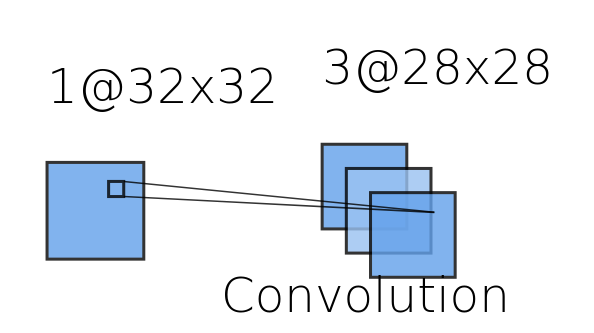
\includegraphics[scale=0.4]{q4_1.png}
                  \end{center}
              \end{mdframed}

        \item
              In given CNN,

              \begin{itemize}
                  \item 32x32 grayscale input images
                  \item Single convolutional layer
                  \item Three 5x5 convolution filters
              \end{itemize}

              To calculate the number of parameters, we have to consider the following:

              \begin{enumerate}
                  \item \textbf{Parameters in Each Filter}: Each 5x5 filter has 5x5 = 25 weight parameters and 1 bias parameter. So, each filter contributes 25 (weights) + 1 (bias) = 26 parameters.

                  \item \textbf{Number of Filters}: three filters in  convolutional layer.
              \end{enumerate}

              Now, calculationg the total number of parameters:
              \begin{align*}
                  \text{Total Parameters} & = (\text{Parameters in Each Filter}) \times (\text{Number of Filters}) \\
                                          & = 26  \times 3                                                         \\
                                          & = 78
              \end{align*}

              So, there are a total of 78 parameters in this CNN model. These parameters include the weights and biases of the three convolution filters.

              \item
               To convert given CNN mondel to ordinary feed-forward neural network we need to keep constraints on
               weights

               Feed-forward nueral network will contain $32 \times 32$ nodes in input layer and and first hidden layer will conatin $28 \times 28 \times 3$ nodes

               weights constraints :
               \begin{itemize}
                \item 
                Pixel in hidden layer image of CNN model(1 pixel) will contain corresponding $5 \times 5$ pixel matrix(25 pixel) in input layer image in CNN model. 
                
                Now in feed-forward neural network we have corresponding nodes for pixel in hidden layer(1 node) and input layer(25).
                
                So for node in hidden layer which is joined to corresponding input layer node other than mentioned 25 nodes having weights as zero

                \item
                So above mentioned 25 pixel(25 nodes) from input layer which is joined to hidden layer node.

                let's consider nodes as $n_1,n_2,n_3,\ldots,n_{25}$. One node in hidden layer will have corresponding 25 nodes in input layer
                for every node in hidden layer

                So weight of $n_k$ of node corresponding node j in hidden layer will have same weight as node $n_k$ of corresponding node i in hidden layer
                from same channel in hidden layer image
               \end{itemize}

               \item
               If there were no constraints, then $32 \times 32 \times 28 \times 28 \times 3$ weights would there
               be in the ordinary feed-forward neural network.
    \end{enumerate}
\end{Solution}
%%%%%%%%%%%%%%%%%%%%%%%%%%%%%%%%%%%%%%%%%%%%%%%%%%%%%%%%%%%%%%%%%%
%New problem
\newpage
\subsubsection*{}
\begin{Problem}
    \textbf{Ch10\_Q6}
\end{Problem}

\begin{Solution}
    \begin{enumerate}[label=\textbf{(\alph*)}]
        \item
              Graph of the function $R(\beta)=sin⁡(\beta)+\frac{\beta}{10}$​ over the range $\beta\epsilon[−6,6]$.

              \begin{center}
                  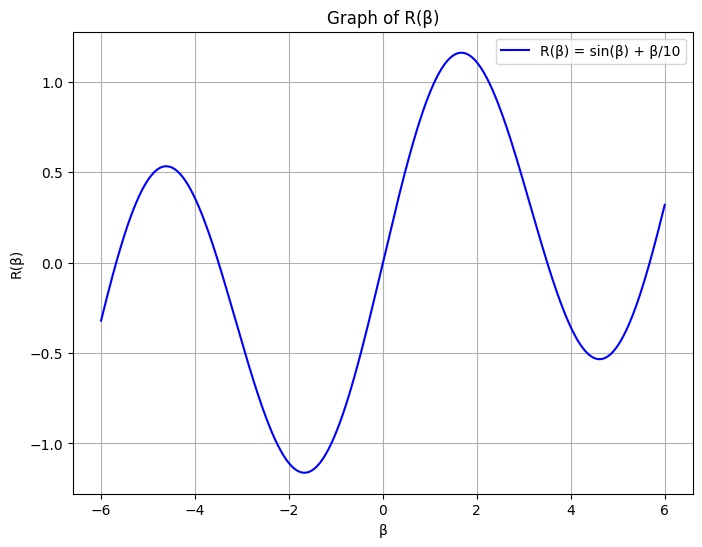
\includegraphics[scale=0.5]{q6_1.png}
              \end{center}
        \item
              The derivative of the function \( R(\beta) = \sin(\beta) + \frac{\beta}{10} \) with respect to \( \beta \)
              \begin{itemize}
                  \item
                        The derivative of \( \sin(\beta) \) with respect to \( \beta \) is \( \cos(\beta) \).
                  \item
                        The derivative of \( \frac{\beta}{10} \) with respect to \( \beta \) is \( \frac{1}{10} \).

              \end{itemize}
              Now, combining these derivatives, we get the derivative of \( R(\beta) \):

              \[
                  R'(\beta) = \cos(\beta) + \frac{1}{10}
              \]

              So, the derivative of the function \( R(\beta) = \sin(\beta) + \frac{\beta}{10} \) is \( R'(\beta) = \cos(\beta) + \frac{1}{10} \).

        \item
              Running a gradient descent to find a local minimum of \( R(\beta) = \sin(\beta) + \frac{\beta}{10} \) with \( \beta_0 = 2.3 \) and a learning rate \( \rho = 0.1 \) involves iteratively updating \( \beta \) using the following formula:

              \[
                  \beta_{i+1} = \beta_i - \rho \cdot \frac{dR}{d\beta}
              \]

              where \( \frac{dR}{d\beta} \) is the derivative of \( R(\beta) \).

              We'll start with \( \beta_0 = 2.3 \) and update it iteratively until convergence.
              \newpage
              \begin{center}
                  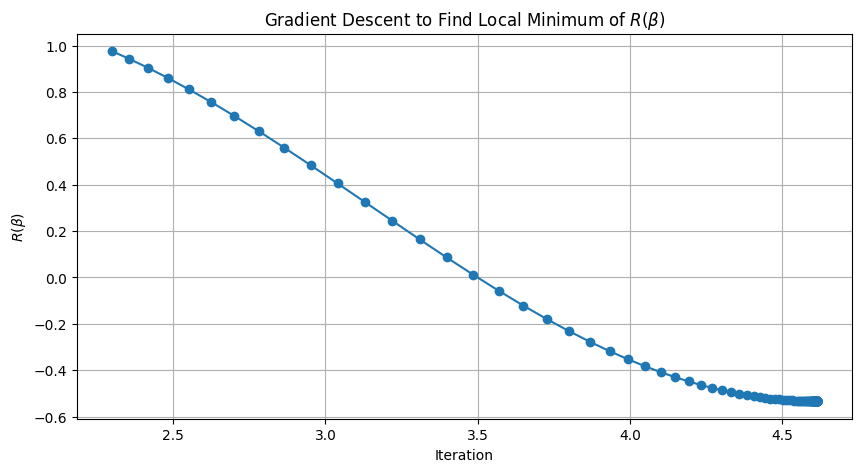
\includegraphics[scale=0.5]{q6_3.png}
              \end{center}

              Final value of $\beta: 4.612220565617592$ \\
              Final value of $R(\beta): -0.5337652811838157$

              So the local minima $R(\beta)=-0.53$ occurs at $\beta = 4.61$ approximately

        \item
              for $B^{o} = 1.4$

              Final value of $\beta: -1.6709610375631647$\\
              Final value of $R(\beta): -1.162083811898611$\\
              So the local minima $R(\beta)=-1.162$ occurs at $\beta = -1.67$ approximately
              \begin{center}
                  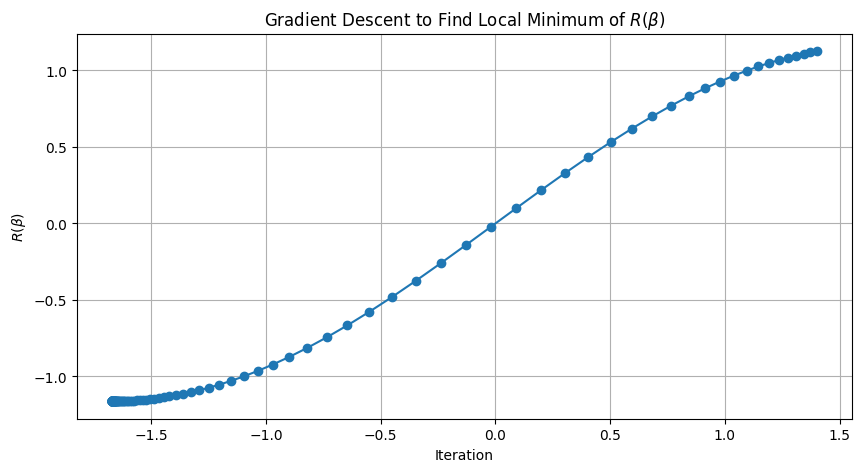
\includegraphics[scale=0.5]{q6_4.png}
              \end{center}
    \end{enumerate}
\end{Solution}

%%%%%%%%%%%%%%%%%%%%%%%%%%%%%%%%%%%%%%%%%%%%%%%%%%%%%%%%%%%%%%%%%%
%Complete the assignment now
\end{document}
%%%%%%%%%%%%%%%%%%%%%%%%%%%%%%%%%%%%%%%%%%%%%%%%%%%%%%%%%%%%%%%%%%
%%%%%%%%%%%%%%%%%%%%%%%%%%%%%%%%%%%%%%%%%%%%%%%%%%%%%%%%%%%%%%%%%%
